\documentclass{article}

% Language setting
% Replace english' with e.g. spanish' to change the document language
\usepackage[english]{babel}

% Set page size and margins
% Replace letterpaper' with a4paper' for UK/EU standard size
\usepackage[letterpaper,top=2cm,bottom=2cm,left=3cm,right=3cm,marginparwidth=1.75cm]{geometry}

% Useful packages
\usepackage{amsmath}
\usepackage{graphicx}
\usepackage[colorlinks=true, allcolors=blue]{hyperref}
\usepackage{array}
\usepackage{longtable}
\usepackage{csquotes}
\usepackage{comment}
\usepackage{booktabs}
\usepackage{tabularx}
\usepackage{listings}
\usepackage{xcolor}
\usepackage{graphicx}
\usepackage{caption}
\usepackage{subcaption}
\usepackage{float}
\usepackage{pdflscape}
\usepackage[toc,page]{appendix}
% Definizione dei colori personalizzati
\definecolor{codegreen}{rgb}{0,0.6,0}
\definecolor{codegray}{rgb}{0.5,0.5,0.5}
\definecolor{codepurple}{rgb}{0.58,0,0.82}
\definecolor{backcolour}{rgb}{0.95,0.95,0.92}
\definecolor{codeblue}{rgb}{0.25,0.5,0.75}
\definecolor{codered}{rgb}{0.75,0.25,0.25}

% Definizione dello stile personalizzato
\lstdefinestyle{mystyle}{
    % backgroundcolor=\color{backcolour},   
    commentstyle=\color{codegreen},
    keywordstyle=\color{magenta},
    numberstyle=\tiny\color{codegray},
    stringstyle=\color{codepurple},
    basicstyle=\ttfamily\footnotesize,
    breakatwhitespace=false,         
    breaklines=true,                 
    captionpos=b,                    
    keepspaces=true,                 
    numbers=left,                    
    numbersep=5pt,                  
    showspaces=false,                
    showstringspaces=false,
    showtabs=false,                  
    tabsize=2
}

% Definizione del linguaggio personalizzato per il codice specifico
\lstdefinelanguage{customjson}{
    morestring=[b]",               % Per interpretare le stringhe
    morekeywords={jtype, identity, label, properties, name, license, softwareType, softwareCategory, presentationDate, subject, object, developedBy}, % Parole chiave
    keywordstyle=\color{magenta},  % Stile delle parole chiave
    sensitive=false,               % Case insensitive
    alsoletter={":,{}"},           % Considera anche i caratteri speciali
    literate=
     *{0}{{{\color{codeblue}0}}}{1} % Colore per i numeri 0-9
      {1}{{{\color{codeblue}1}}}{1}
      {2}{{{\color{codeblue}2}}}{1}
      {3}{{{\color{codeblue}3}}}{1}
      {4}{{{\color{codeblue}4}}}{1}
      {5}{{{\color{codeblue}5}}}{1}
      {6}{{{\color{codeblue}6}}}{1}
      {7}{{{\color{codeblue}7}}}{1}
      {8}{{{\color{codeblue}8}}}{1}
      {9}{{{\color{codeblue}9}}}{1}
      {:}{{{\color{codered}:}}}{1} % Colore per i due punti
      {,}{{{\color{codered},}}}{1} % Colore per le virgole
      {\{}{{{\color{orange}{\{}}}}{1} % Colore per parentesi graffe aperte
      {\}}{{{\color{orange}{\}}}}}{1}, % Colore per parentesi graffe chiuse
}

% Define a custom language style for JSON
\lstdefinelanguage{json}{
    literate=
     *{0}{{{\color{blue}0}}}{1} % Colors for numbers
      {1}{{{\color{blue}1}}}{1}
      {2}{{{\color{blue}2}}}{1}
      {3}{{{\color{blue}3}}}{1}
      {4}{{{\color{blue}4}}}{1}
      {5}{{{\color{blue}5}}}{1}
      {6}{{{\color{blue}6}}}{1}
      {7}{{{\color{blue}7}}}{1}
      {8}{{{\color{blue}8}}}{1}
      {9}{{{\color{blue}9}}}{1}
      {:}{{{\color{red}:}}}{1} % Colors for colons
      {,}{{{\color{red},}}}{1} % Colors for commas
      {\{}{{{\color{orange}{\{}}}}{1} % Colors for braces
      {\}}{{{\color{orange}{\}}}}}{1},
}


\lstset{style=mystyle}

\title{S2R-Wind: Semi-Supervised Regression on Wind Power Forecasting}

\author{Nicolas Pinto - Student ID: 807348 \\\href{https://github.com/npinto97/S2R-Wind}{https://github.com/npinto97/S2R-Wind}}
\date{A.Y. 2024-2025}

\begin{document}
\maketitle

\section{Introduction}
Wind power forecasting is a critical task for the operation and integration of renewable energy into the electrical grid. However, obtaining labeled data for training predictive models, such as actual power output (PATV) measurements, is expensive and limited in practice. In contrast, large volumes of unlabeled sensor data are typically available from wind turbines. This imbalance motivates the use of \textit{semi-supervised learning (SSL)} techniques that can leverage both labeled and unlabeled instances to improve performance.

This project investigates the application of semi-supervised regression methods on a realistic wind turbine dataset derived from the Baidu KDD Cup 2022\footnote{\href{https://aistudio.baidu.com/competition/detail/152/0/introduction}{https://aistudio.baidu.com/competition/detail/152/0/introduction}}. Our aim is to evaluate how effectively SSL models can improve forecasting performance when labeled data is scarce, and to benchmark these models against strong supervised baselines.

We focus primarily on \textbf{S2RMS}, a co-training-based ensemble SSL framework developed in Python, and compare it against a state-of-the-art tree-based SSL method implemented in \textbf{CLUS+}, a decision tree learner supporting predictive clustering trees (PCTs) with semi-supervised extensions. We further include \textbf{ElasticNet} and \textbf{XGBoost} as supervised baselines, enabling a rigorous comparative evaluation.

To ensure fairness and reproducibility, all models are trained and evaluated across eight temporal folds with varying percentages (10\%, 20\%, 70\%) of labeled data. The training, evaluation, and data generation processes follow a standardized pipeline aligned with the CRISP-DM methodology. Performance is measured using RMSE, MAE, RSE, and R$^2$, with additional analyses on the influence of label availability and model robustness.

The remainder of this document describes the methodological pipeline, models, and results in detail, offering a data-driven perspective on the utility and limitations of semi-supervised learning in practical wind power prediction settings.


\section{Business Understanding}
Wind energy providers require accurate short-term power forecasts to support grid stability, market bidding, and asset management. Forecasting models must estimate the turbine's active power output (PATV) using historical sensor measurements, meteorological variables, and temporal features. However, collecting labeled output data at high quality and for extended periods is costly. In contrast, input data is generally abundant and not expensive to obtain.

This scenario defines a typical semi-supervised regression setting, where only a subset of instances contains ground truth labels. The business goal is to maximize predictive accuracy using minimal labeled data, reducing annotation costs while maintaining forecast reliability.

To simulate realistic deployment conditions, we adopt a rolling-window temporal evaluation strategy with eight time-based folds, each comprising 15 days of training and 7 days of testing. Within each fold, only a fraction of the training samples are labeled (10\%, 20\%, or 70\%), while the remainder are unlabeled.

Forecasting accuracy is evaluated using multiple metrics. RMSE provides a scale-sensitive view of absolute error, while MAE offers robustness to outliers. RSE quantifies the error relative to variance in the ground truth and R$^2$ indicates the proportion of variance explained by the model.

\section{Data Understanding}
This work builds upon a dataset released as part of the Baidu KDD Cup 2022 wind power forecasting challenge, featuring high-frequency SCADA (Supervisory Control and Data Acquisition) data from 134 wind turbines owned by Longyuan Power Group. Measurements are recorded every 10 minutes over 245 consecutive days, capturing both operational and environmental conditions of each turbine at a given timestamp. The resulting data forms a dense multivariate time series with rich temporal and spatial structure.

Each row in the dataset includes the turbine identifier (\texttt{TurbID}), a day index (\texttt{Day}), and a timestamp (\texttt{Tmstamp}), alongside 13 numerical signals. These include meteorological variables such as wind speed (\texttt{Wspd}), wind direction (\texttt{Wdir}), external and internal temperatures (\texttt{Etmp}, \texttt{Itmp}), as well as machine state indicators like nacelle yaw angle (\texttt{Ndir}), blade pitch angles (\texttt{Pab1}, \texttt{Pab2}, \texttt{Pab3}), reactive power (\texttt{Prtv}), and the primary output variable, active power (\texttt{Patv}). A separate metadata file provides the GPS coordinates of each turbine, enabling spatial analysis if desired.

\begin{figure}[h]
    \centering
    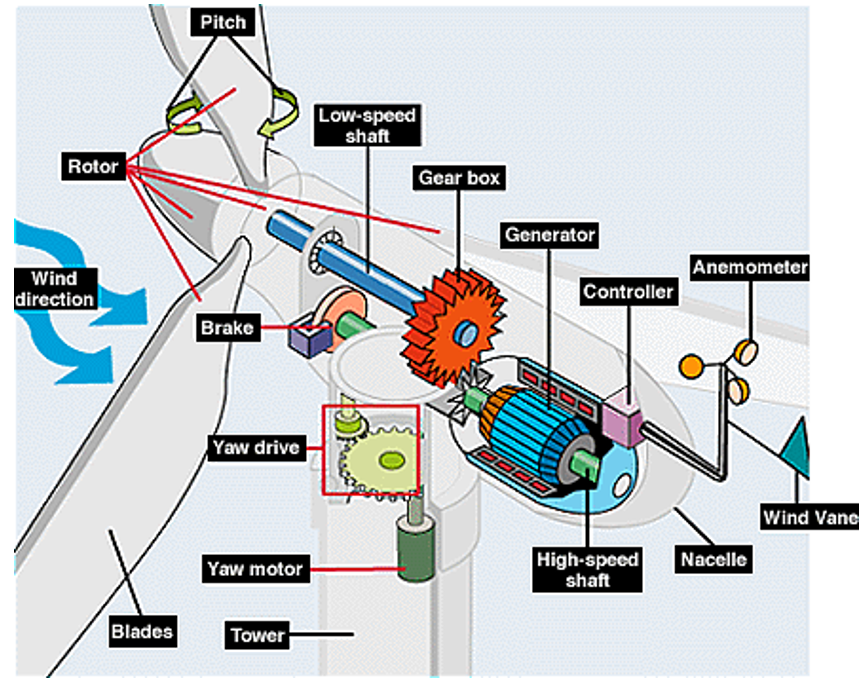
\includegraphics[width=0.7\textwidth]{figures/turbine.png}
    \caption{\url{https://en.wikipedia.org/wiki/File:EERE_illust_large_turbine.gif}}
    \label{fig:turbine}
\end{figure}

To balance complexity with computational feasibility, we restricted our analysis to a representative subset of 10 turbines. This allowed us to maintain the dataset’s temporal and spatial variability while keeping training and evaluation times manageable.


The forecasting task focuses on predicting the short-term future value of \texttt{Patv}. To formalize this as a supervised regression problem, the target was renamed \texttt{patv\_target\_1}, indicating a 10-minute prediction horizon. We also derived several time-based features—such as hour, minute, and day of the week—from each timestamp to help capture cyclical or calendar-related patterns.

To assess generalization over time, we adopted a \textit{temporally stratified cross-validation} strategy. The data was split into eight non-overlapping folds, where each fold consists of 15 consecutive days for training and 7 subsequent days for testing. This simulates deployment scenarios in which models must predict unseen future intervals, accounting for shifts in turbine behavior or weather conditions over time.

Key preprocessing steps were applied before modeling. Missing values in the patv series were filled using forward- and backward-filling, based on the assumption that short-term continuity in power output is a valid approximation. Then, for each turbine, we computed lagged values of \texttt{patv\_target\_1} over a 12-step window (equivalent to two hours of history), allowing models to leverage autoregressive signals. Additionally, lead values were created to define the target outputs in a supervised learning setup.

The resulting dataset consists entirely of numerical features, making it suitable for a variety of learning algorithms, from linear regression to tree ensembles and neural networks. Prior to training, feature scaling was performed using \texttt{StandardScaler} from \texttt{scikit-learn}, fitted only on the training data of each fold and consistently applied to the corresponding test set.

For semi-supervised experiments, we simulated limited-label settings by subsampling 10\%, 20\%, or 70\% of the training data as labeled, while treating the rest as unlabeled. S2RMS leverages these unlabeled examples through iterative pseudo-labeling. CLUS+, on the other hand, handles them natively via symbolic missing targets during model construction. It's important to note that for CLUS experiments, the same fold structure is reused, but without applying external normalization, since the CLUS framework includes its own internal scaling mechanisms. In contrast, supervised baselines like ElasticNet and XGBoost rely on the externally scaled features and are trained only on the labeled subset.

A detailed overview of the dataset structure, including the differences between the original full dataset and the reduced per-fold setting, is provided in Table~\ref{tab:dataset-comparison}.

% \begin{table}[h]
% \centering
% \caption{Dataset summary statistics across folds and supervision levels.}
% \label{tab:dataset-summary}
% \begin{tabularx}{\textwidth}{X r}
% \toprule
% \textbf{Metric} & \textbf{Value} \\
% \midrule
% Lagged Feature Dimensionality & 12 \\
% Total Features (after lag/lead) & 17 \\
% \# Labeled Instances (10\%) & 2,304 \\
% \# Unlabeled Instances (10\%) & 20,736 \\
% \# Labeled Instances (20\%) & 4,608 \\
% \# Unlabeled Instances (20\%) & 18,432 \\
% \# Labeled Instances (70\%) & 16,127 \\
% \# Unlabeled Instances (70\%) & 6,912 \\
% \bottomrule
% \end{tabularx}
% \end{table}

\begin{table}[ht]
\centering
\caption{Comparison between the original dataset and the reduced per-fold version used in experiments.}
\label{tab:dataset-comparison}
\renewcommand{\arraystretch}{1.2}
\begin{tabularx}{\textwidth}{l X X}
\toprule
\textbf{Property} & \textbf{Original Dataset} & \textbf{Per-Fold Dataset} \\
\midrule
Time Span & 245 consecutive days & 22 days (15 for training, 7 for testing) \\
Turbines & 134 & 10 \\
Sampling Frequency & 10 minutes & 10 minutes \\
Total Instances & $\sim$4.7 million & 33,120 per fold \\
Instances per Fold & -- & 23,040 for training \newline 10,080 for testing \\
Labeled Samples (10\%) & -- & $\sim$2,300 \\
Labeled Samples (20\%) & -- & $\sim$4,600 \\
Labeled Samples (70\%) & -- & $\sim$16,000 \\
Unlabeled Samples & -- & 23,040 - Labeled Samples \\
Features & 19 numerical + 1 target & Same \\
Target Variable & PATV & Same \\
\bottomrule
\end{tabularx}
\end{table}


\section{Data Preparation}
The raw SCADA dataset underwent a structured transformation pipeline to prepare it for both supervised and semi-supervised regression tasks. This process involved time-based feature engineering, instance windowing, normalization, and formatting into formats compatible with distinct modeling environments, such as Python-based libraries (e.g., scikit-learn, XGBoost) and the Java-based CLUS+ framework.

A critical step in preprocessing was the construction of lagged features: for each instance, the 12 preceding values of \texttt{patv\_target\_1} were appended as predictors, yielding a temporally contextualized representation of turbine output. The prediction target was the next time step (i.e., 10 minutes ahead), preserving the causal structure essential for real-time forecasting applications. These feature transformations were computed independently per turbine to maintain intra-series temporal coherence.

From the processed data, two parallel sets of folds were derived. The first set, comprising scaled folds, was used for all Python-based methods—ElasticNet, XGBoost, and S2RMS. Here, both input features and targets were normalized using a \texttt{StandardScaler}, fitted on the training portion of each fold. These scalers were stored and reused consistently for testing and for inverse transforming predictions during evaluation. The second set, based on unscaled data, was generated specifically for CLUS+, which performs its own internal normalization during model induction. This separation ensures consistency with the modeling assumptions of each framework.

Each fold consists of a 15-day training window and a subsequent 7-day test window. Within each training fold, three supervised signal levels were simulated by marking 10%, 20%, or 70% of the training data as labeled. For semi-supervised configurations, the remaining samples were considered unlabeled. In the CLUS+ folds, unlabeled examples were explicitly encoded by replacing their target values with \texttt{?}, allowing CLUS+ to interpret them as partially observed during the construction of Predictive Clustering Trees (PCTs). For S2RMS, labeled and unlabeled examples were kept distinct and processed through a dedicated pseudo-labeling pipeline during training.

All folds were exported in both CSV and ARFF formats. CSV was used exclusively with ElasticNet and XGBoost, while ARFF was required for both CLUS+ and S2RMS. The dual-format export and fold parallelism ensured that all models were trained and evaluated on an identical temporal and structural basis, thus enabling fair comparative analysis.


\section{Modeling}
Three classes of models were implemented and evaluated: supervised baselines (ElasticNet, XGBoost), a semi-supervised co-training approach (S2RMS), and a decision tree-based semi-supervised ensemble method (CLUS+). All models were trained independently on each fold and for each label percentage, maintaining identical data splits for fairness.

\subsection{Supervised Baselines}

The \textit{ElasticNet} model was implemented using a scikit-learn pipeline with standard scaling and a grid search over regularization parameters. The training set consisted only of labeled data. Hyperparameters were selected using time series-aware cross-validation (5 splits). ElasticNet was chosen as a linear baseline, known for its robustness under small sample sizes due to its \texttt{l1\_ratio} control over sparsity.

The \textit{XGBoost} baseline was trained similarly, using a grid search over tree depth, learning rate, and number of estimators. XGBoost offers a strong nonlinear baseline and often outperforms other methods when sufficient labeled data is available. GPU acceleration was enabled during both training and inference using the \texttt{device=cuda} and \texttt{tree\_method=hist} parameters. Predictions were made after applying the inverse transform of the target scaler.

Both baseline methods were trained exclusively on the labeled portion of the data, entirely ignoring the unlabeled training samples. As such, they serve as upper-bound reference points for evaluating the effectiveness of semi-supervised models. Their performance represents what can be achieved under fully supervised conditions, assuming access only to annotated data. This allows us to assess whether semi-supervised techniques like S2RMS and CLUS+ can approach or surpass these upper bounds by effectively leveraging additional unlabeled information.

\subsection{S2RMS}

The \textit{S2RMS} framework \cite{liu2024semi} (Semi-Supervised Regression via Embedding Space Mapping and Pseudo-Label Smearing) extends classical co-training by combining deep metric learning with a cautious pseudo-labeling mechanism tailored for regression tasks. At its core, S2RMS employs a Triplet neural network trained on pairwise data constructed from the labeled set, enabling the projection of both labeled and unlabeled instances into a learned embedding space. This mapping encourages smoothness and local consistency under the manifold assumption, such that similar instances lie closer in the latent space. In our implementation, we use three heterogeneous XGBoost regressors as base learners, each initialized on a distinct 80\% bootstrap sample of the labeled data, with the remaining 20\% reserved for internal validation.

During each co-training round, the Triplet network is used to identify unlabeled instances that are highly similar to labeled ones, according to an exponentially decaying similarity threshold $\tau$, and these are aggregated into a candidate pool. Each regressor consults the predictions from the other two regressors to compute the variance (or standard deviation) of the outputs, which acts as a stability criterion. Only instances with a standard deviation below a fixed threshold (set to 0.4) are considered sufficiently stable for pseudo-labeling, a technique inspired by the "pseudo-label smearing" strategy proposed by Liu et al. To manage computational load, we limit each learner to at most 500 such candidates per iteration.

A margin-based confidence metric, the $\Delta$-score, is then calculated for each stable sample, quantifying its utility by measuring the expected reduction in validation error (MSE) after hypothetical inclusion. Only the top $g\_r$ samples per learner, those demonstrating positive gain, are accepted into the training set per iteration. This highly selective acquisition procedure mitigates the risk of error propagation due to noisy pseudo-labels, effectively controlling for label drift.

The embedding-based similarity selection is governed by a decaying schedule $\tau_{t+1} = \lambda \tau_t$ (with $\lambda < 1$), allowing the algorithm to begin conservatively by focusing on near-neighbors and gradually relax this constraint in later stages. This mimics a curriculum learning approach by progressively exposing learners to more diverse samples. After each augmentation, regressors are retrained from scratch to preserve independence among learners and to ensure proper integration of the new data.

Final predictions are obtained via ensemble averaging. To support efficient inference, particularly at scale, GPU-accelerated prediction paths are utilized when available via the XGBoost backend, while maintaining CPU compatibility to ensure cross-platform reproducibility and robustness.


\subsection{CLUS+}

The \textit{CLUS+} framework \cite{petkovic2023clusplus} is a Java-based open-source machine learning system built upon the predictive clustering paradigm, specifically designed for structured output prediction. It extends the original CLUS software with advanced support for semi-supervised learning, ensemble methods, and feature importance analysis. At its core, CLUS+ utilizes Predictive Clustering Trees (PCTs), which generalize classical decision trees by treating the decision process as a top-down clustering operation. Each internal node partitions the data based on a variance reduction criterion tailored to the task (e.g., single-target or multi-target regression), while leaf nodes represent clusters labeled by prototype functions. These PCTs are trained using a top-down induction-of-decision-trees (TDIDT) algorithm with a greedy heuristic that maximizes homogeneity of the induced clusters.

In our experiments, CLUS+ was employed in its ensemble-based semi-supervised mode by enabling the \texttt{-forest -ssl} flags in the settings file. This configuration constructs a Random Forest of PCTs using bootstrap aggregating (bagging) and random feature subspace selection at each node. The number of trees in the ensemble and the function $f(D)$, which controls the subspace size (typically set to $\sqrt{D}$), are user-defined. To support partially labeled data, the SSL component of CLUS+ implements self-training within the predictive clustering framework. It allows trees to be grown even when instances contain missing target values, making it highly applicable to real-world scenarios with sparse annotations.

The experimental workflow included automatic generation of settings files for each fold and supervision level (Listing~\ref{lst:clus_settings}). These configuration files define paths to training and testing datasets in ARFF format, SSL-specific parameters, and the choice of feature ranking method, Genie3 in our case. Genie3 is an ensemble-based feature importance estimator inspired by Random Forests, adapted to structured output settings. When enabled, feature importance scores are output to \texttt{.fimp} files, including detailed rankings for each predictive target.

\begin{lstlisting}[label=lst:clus_settings, caption=CLUS+ Settings File Example for the Fold0 with 10\% Labeled Data]
[General]
RandomSeed = 42

[Data]
File = .data/swdpf/clus_ssl_arffs\fold0_ssl_10.arff
TestSet = .data/swdpf/clus_ssl_arffs\fold0_test.arff
PruneSet = None

[Attributes]
Descriptive = 1-19
Target = 20

[Tree]
Heuristic = VarianceReduction

[Ensemble]
SelectRandomSubspaces = SQRT
EnsembleMethod = RForest
FeatureRanking = Genie3
Iterations = 10 

[SemiSupervised]
SemiSupervisedMethod = PCT

[Output]
WritePredictions = Train, Test

\end{lstlisting}

Each execution of CLUS+ yields a comprehensive \texttt{.out} file summarizing the parameter settings, model variants (baseline, original full tree, pruned version), and evaluation metrics such as RMSE, MAE, and RSE on both training and test data. The \texttt{.train.pred.arff} and \texttt{.test.pred.arff} files record the instance-level predictions, including both ground truth and ensemble-averaged outputs, along with auxiliary metadata such as contributing models and prediction confidence.

To streamline result collection, a custom parser was used to automatically extract model statistics from the CLUS+ outputs, aggregating them across folds and supervision levels. The experimental configuration utilized variance reduction as the split criterion, random subspace selection (SQRT) for node-wise feature selection, and an ensemble size of ten trees per forest. This setup offered a robust trade-off between interpretability, scalability, and predictive performance, while maintaining compatibility with structured output learning and semi-supervised settings.


\section{Evaluation}
We evaluate the performance of S2RMS against two baseline models, ElasticNet and XGBoost, across multiple folds and varying levels of supervision. The evaluation metrics include Root Mean Squared Error (RMSE), Mean Absolute Error (MAE), Relative Squared Error (RSE), and Coefficient of Determination (R$^2$). These are computed over 8 stratified temporal folds, using 10\%, 20\%, and 70\% of labeled data for training. The remaining data in each fold is held out for testing.

\subsection{Overview of Experimental Setup}

For each fold, labeled and unlabeled sets are selected proportionally from the available data. The Table~\ref{tab:training_samples} shows the average number of labeled and unlabeled instances used in training and testing, respectively. The semi-supervised method, S2RMS, leverages additional unlabeled data in training, while ElasticNet and XGBoost rely solely on the labeled portion.

\begin{table}[ht]
\centering
\caption{Mean number of labeled and unlabeled training samples per model and scale.}
\label{tab:training_samples}
\renewcommand{\arraystretch}{1.2}
\begin{tabularx}{\textwidth}{l c *{4}{>{\centering\arraybackslash}X}}
\toprule
Model & Scale & Labeled & Unlabeled & $n_{\text{train}}$ & $n_{\text{test}}$ \\
\midrule
CLUS+       & 10  & 2304  & 20736 & 23040 & 10080 \\
CLUS+       & 20  & 4608  & 18432 & 23040 & 10080 \\
CLUS+       & 70  & 16127 & 6913  & 23040 & 10080 \\
ElasticNet  & 100 & 23040 & --    & 23040 & 10080 \\
S2RMS       & 10  & 2304  & 20736 & 23040 & 10080 \\
S2RMS       & 20  & 4608  & 18432 & 23040 & 10080 \\
S2RMS       & 70  & 16127 & 6913  & 23040 & 10080 \\
XGBoost     & 100 & 23040 & --    & 23040 & 10080 \\
\bottomrule
\end{tabularx}
\end{table}

Across all scales, CLUS+ consistently outperforms both S2RMS and ElasticNet. When trained with only 10\% of the labeled data, CLUS+ achieves an average RMSE of approximately 135.18, with an $R^2$ of 0.882. In contrast, S2RMS underperforms significantly at this scale, with an RMSE of 197.74 and an $R^2$ of 0.733. This performance gap narrows only slightly at higher label densities. Even at 70\% labeled data, CLUS+ maintains superiority with an RMSE of 130.09 and $R^2$ of 0.891, while S2RMS does not scale comparably.

Notably, CLUS+ shows a reduction in both error metrics and variance as the proportion of labeled data increases from 10\% to 20\%, which aligns with expectations in semi-supervised learning. However, the marginal improvement from 20\% to 70\% is modest, suggesting that CLUS+ extracts considerable predictive value even from limited labeled supervision. This behavior is characteristic of its decision tree-based semi-supervised architecture, which can effectively leverage unlabeled instances by exploiting structural regularities in the input space.

ElasticNet, trained using fully labeled data (100\% of the training set), delivers the best raw RMSE (121.11) and lowest MAE (77.38). However, it lacks the semi-supervised capability and requires full annotation, making it unsuitable in label-scarce scenarios. Moreover, the minimal performance advantage of ElasticNet compared to CLUS+ at 70\% labeled data illustrates that CLUS+ provides a more scalable and label-efficient alternative, especially considering its performance at lower annotation budgets.

S2RMS performs consistently below both CLUS+ and ElasticNet. Its RMSE remains high and unstable across scales, and even at 70\%, it fails to match CLUS+'s performance at 10\%. The method's iterative pseudo-labeling and model update strategy introduces variance in fold-level results. One possible cause is that its candidate selection process and pseudo-labeling quality are strongly affected by the initial label distribution, which can degrade model reliability when the sample size is small or the feature space is high-dimensional.

\begin{table}[ht]
\centering
\caption{Mean of RMSE, MAE, RSE, and $R^2$ per model and scale.}
\renewcommand{\arraystretch}{1.2}
\begin{tabularx}{\textwidth}{l c *{8}{>{\centering\arraybackslash}X}}
\toprule
Model & Scale & RMSE$_\mu$ & MAE$_\mu$ & RSE$_\mu$ & $R^2_\mu$\\
\midrule
CLUS+       & 10    & 135.18    & 90.91     & 0.13  & 0.88 \\
CLUS+       & 20    & 126.08    & 81.92     & 0.11  & \textbf{0.90} \\
CLUS+       & 70    & 130.09    & 90.05     & 0.12  & 0.89 \\
ElasticNet  & 100   & \textbf{121.11}    & \textbf{77.38}     & \textbf{0.10}   & \textbf{0.90}\\
S2RMS       & 10    & 197.74    & 140.82    & 0.27  & 0.73 \\
S2RMS       & 20    & 191.82    & 135.77    & 0.25  & 0.75 \\
S2RMS       & 70    & 187.34    & 131.48    & 0.24  & 0.76 \\
XGBoost     & 100   & 152.46    & 101.78    & 0.15  & 0.85\\
\bottomrule
\end{tabularx}
\end{table}

For a visual comparison of these metrics across models and labeling scales, refer to the plots provided in Appendix~\ref{sec:appendix_metrics}.
For the detailed performance metrics for each fold, model, and labeling scale, refer to the plots provided in Appendix~\ref{app:detailed_results}.

\subsection{Computational Efficiency}

In addition to delivering superior predictive performance, CLUS+ offers significant advantages in computational efficiency. Training S2RMS on a full fold using only 10\% of labeled data often resulted in excessive memory consumption and prolonged runtimes, frequently exceeding available system resources despite aggressive parallelization and GPU acceleration. To mitigate this, we were forced to limit the candidate set used during pseudo-labeling and adapt the base regressors to GPU-compatible implementations. Even with these adjustments, the training process remained substantially slower than that of CLUS+. This behavior is consistent with the original experimental design in the S2RMS paper, where all evaluations were conducted on considerably smaller datasets—typically in the order of a few thousand instances. In particular, S2RMS was applied to a random subset of 2000 data points\cite{liu2024semi}, rather than to the full data distribution, which masks the method’s poor scalability under realistic data volumes. In contrast, CLUS+ is able to operate on the full training set without any reduction, maintaining both accuracy and tractable training times. This makes CLUS+ not only more accurate, but also vastly more practical for large-scale or time-sensitive applications

% \section{Discussion}
% \input{contents/discussion}

\section{Conclusion}
This study explored the effectiveness of semi-supervised regression models for wind power forecasting under varying degrees of label scarcity. Using a realistic SCADA dataset with over 20,000 training instances per fold, we evaluated three modeling strategies: a co-training-based ensemble method (S2RMS), a decision tree-based semi-supervised learner (CLUS+), and two fully supervised baselines (ElasticNet and XGBoost). Experiments were performed across eight temporal folds and multiple labeled data proportions (10\%, 20\%, 70\%).

The results demonstrate that CLUS+ consistently delivers superior predictive performance among the semi-supervised methods. At just 20\% labeled data, CLUS+ matches or exceeds the accuracy of fully supervised baselines trained on the entire dataset. This level of efficiency is critical in operational settings where labeling is costly or infeasible at scale. Its ability to robustly integrate unlabeled instances, without requiring aggressive pseudo-labeling or iterative retraining, makes it particularly effective in high-dimensional, time-dependent domains such as wind power prediction.

In contrast, S2RMS exhibited unstable and subpar performance across all scales. Despite modifications to improve efficiency, such as restricting candidate sets and leveraging GPU acceleration, S2RMS failed to generalize reliably. Its high computational cost and memory usage further undermine its practicality. These shortcomings align with the original S2RMS design, which was validated on small-scale datasets of only 2,000 examples per run. When scaled to realistic data volumes, the method struggles to maintain performance and tractability.

CLUS+ also excels in terms of computational efficiency. It trains significantly faster than S2RMS while maintaining its predictive strength across a wide range of label budgets. The method’s native support for symbolic missing values, ensemble-based architecture, and minimal reliance on hyperparameter tuning make it an attractive candidate for real-world deployments.

Overall, this work confirms the practical viability of semi-supervised tree ensembles for large-scale wind power forecasting. In particular, CLUS+ emerges as a scalable, accurate, and resource-efficient solution, outperforming both traditional supervised baselines and modern SSL alternatives when evaluated under realistic constraints.


\begin{appendices}
\section{Performance Metrics by Model and Labeling Scale}
\label{sec:appendix_metrics}
These results clearly show that CLUS+, through its ensemble-based semi-supervised approach, achieves the best balance between label efficiency and predictive performance. It is especially well-suited for wind power forecasting scenarios where labeled data is expensive or partially missing.

\begin{figure}[!ht]
    \centering
    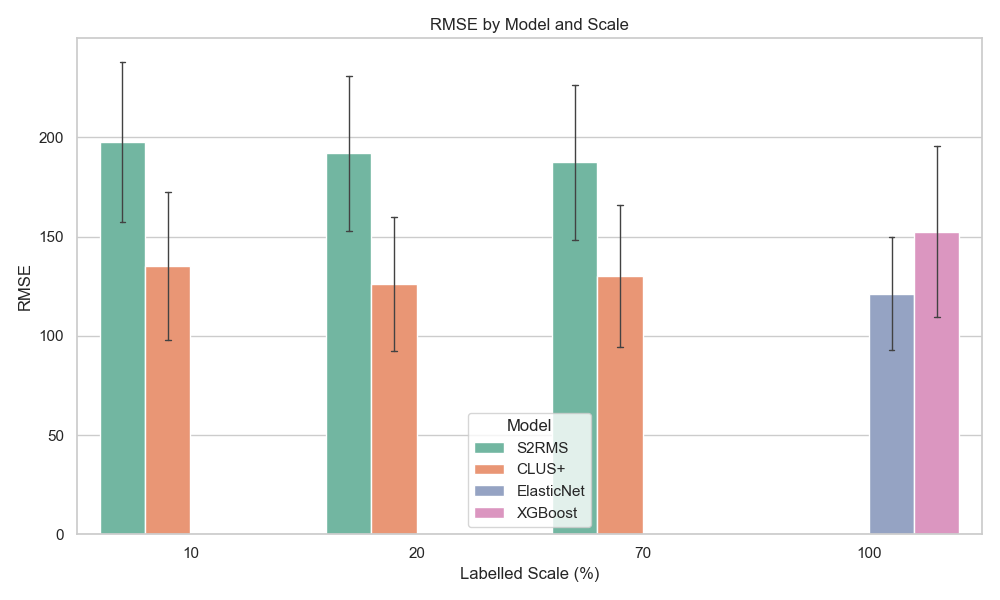
\includegraphics[width=0.7\textwidth]{figures/rmse_by_model_and_scale.png}
    \caption{RMSE by model and scale}
    \label{fig:rmse}
\end{figure}
\begin{figure}[!ht]
    \centering
    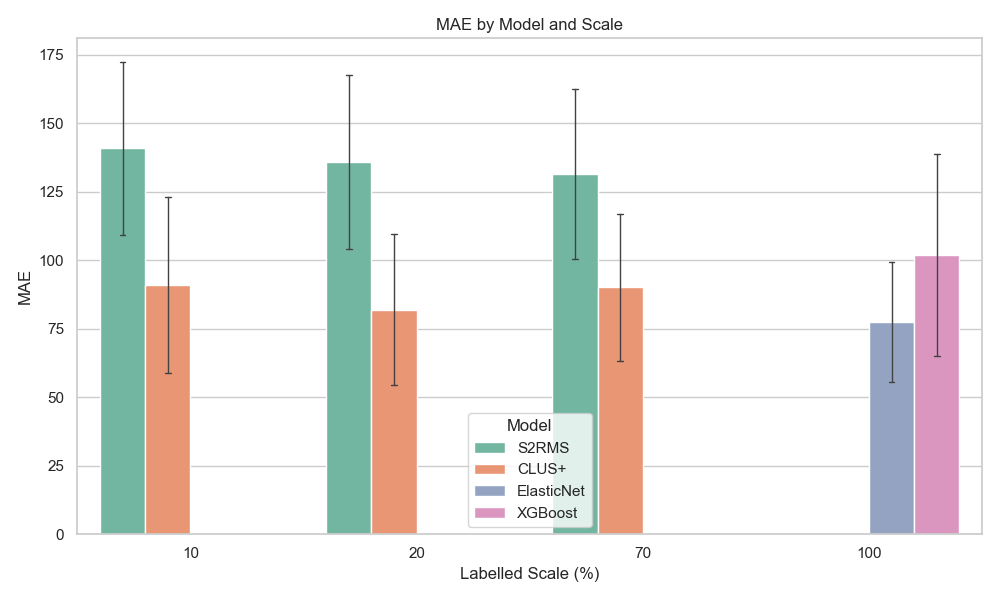
\includegraphics[width=0.7\textwidth]{figures/mae_by_model_and_scale.png}
    \caption{MAE by model and scale}
    \label{fig:mae}
\end{figure}
\begin{figure}[!ht]
    \centering
    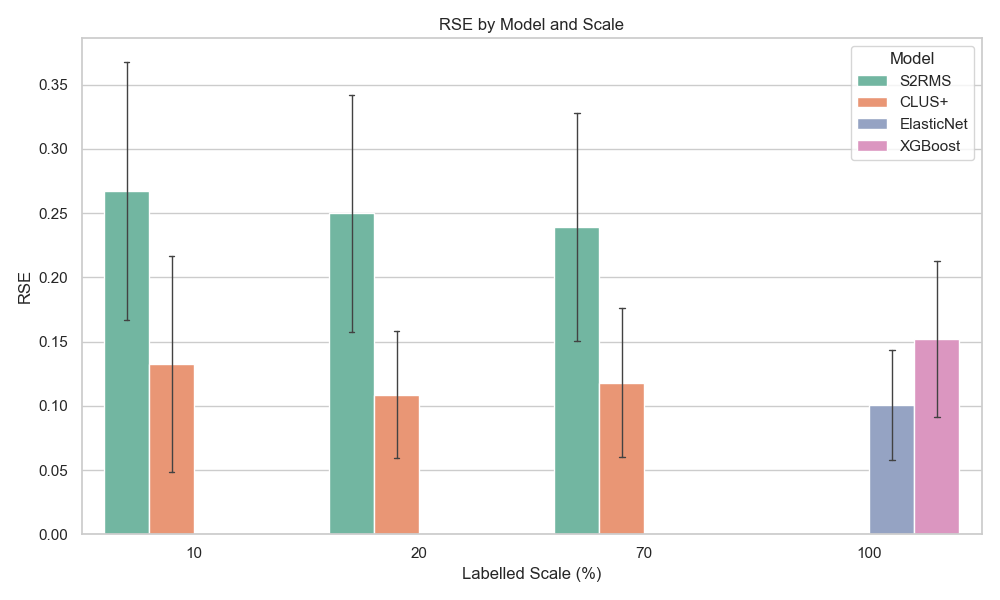
\includegraphics[width=0.7\textwidth]{figures/rse_by_model_and_scale.png}
    \caption{RSE by model and scale}
    \label{fig:rse}
\end{figure}
\begin{figure}[!ht]
    \centering
    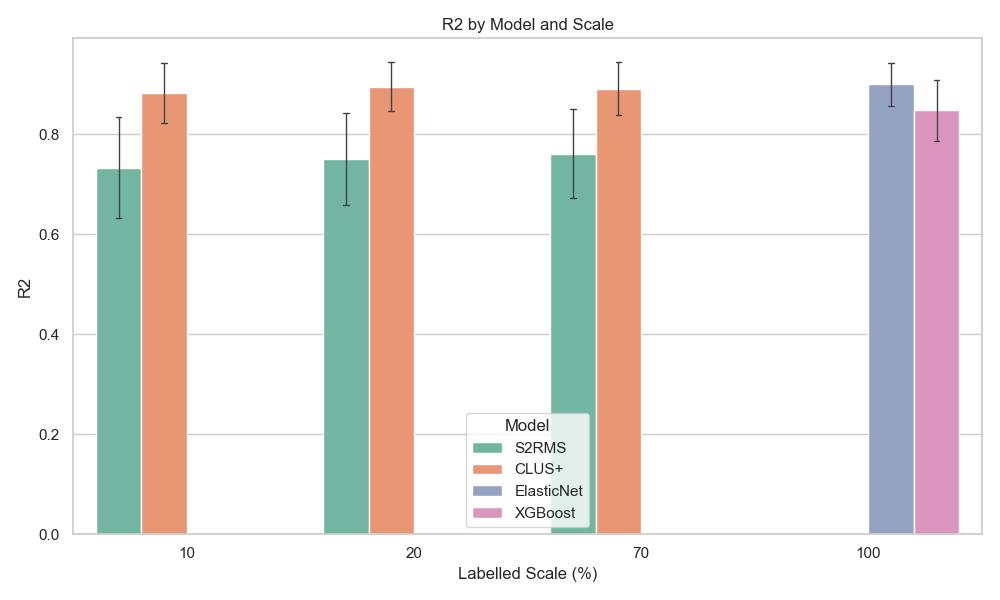
\includegraphics[width=0.7\textwidth]{figures/r2_by_model_and_scale.png}
    \caption{$R^2$ by model and scale}
    \label{fig:r2}
\end{figure}

\newpage
\section{Detailed Results per Fold and Model}
\label{app:detailed_results}

\noindent
This appendix reports the detailed performance metrics for each fold, model, and labeling scale.

%\renewcommand{\arraystretch}{1.1} % aumenta lo spazio tra le righe
\begin{longtable}{l c c c c c c c c c c}
\toprule
\textbf{Model} & \textbf{fold} & \textbf{scale} & \textbf{rmse} & \textbf{mae} & \textbf{rse} & \textbf{$R^2$} & \textbf{n\_lab} & \textbf{n\_unlab} & \textbf{n\_train} & \textbf{n\_test} \\
\midrule
S2RMS & 0 & 10 & 245.65 & 177.61 & 0.28 & 0.72 & 2304 & 20736 & 23040 & 10080 \\ 
S2RMS & 1 & 10 & 200.46 & 150.13 & 0.43 & 0.57 & 2304 & 20736 & 23040 & 10080 \\ 
S2RMS & 2 & 10 & 121.72 & 78.8 & 0.2 & 0.8 & 2304 & 20736 & 23040 & 10080 \\ 
S2RMS & 3 & 10 & 155.65 & 110.85 & 0.1 & 0.9 & 2304 & 20736 & 23040 & 10080 \\ 
S2RMS & 4 & 10 & 220.72 & 163.23 & 0.25 & 0.75 & 2304 & 20736 & 23040 & 10080 \\ 
S2RMS & 5 & 10 & 225.86 & 155.3 & 0.33 & 0.67 & 2304 & 20736 & 23040 & 10080 \\ 
S2RMS & 6 & 10 & 204.02 & 142.03 & 0.22 & 0.78 & 2304 & 20736 & 23040 & 10080 \\ 
S2RMS & 7 & 10 & 207.81 & 148.57 & 0.32 & 0.68 & 2304 & 20736 & 23040 & 10080 \\ 
S2RMS & 0 & 20 & 229.06 & 163.76 & 0.24 & 0.76 & 4608 & 18432 & 23040 & 10080 \\ 
S2RMS & 1 & 20 & 193.37 & 142.66 & 0.4 & 0.6 & 4608 & 18432 & 23040 & 10080 \\ 
S2RMS & 2 & 20 & 112.29 & 70.23 & 0.17 & 0.83 & 4608 & 18432 & 23040 & 10080 \\ 
S2RMS & 3 & 20 & 154.47 & 107.98 & 0.1 & 0.9 & 4608 & 18432 & 23040 & 10080 \\ 
S2RMS & 4 & 20 & 220.38 & 163.37 & 0.25 & 0.75 & 4608 & 18432 & 23040 & 10080 \\ 
S2RMS & 5 & 20 & 210.49 & 140.98 & 0.29 & 0.71 & 4608 & 18432 & 23040 & 10080 \\ 
S2RMS & 6 & 20 & 209.85 & 150.67 & 0.23 & 0.77 & 4608 & 18432 & 23040 & 10080 \\ 
S2RMS & 7 & 20 & 204.61 & 146.53 & 0.31 & 0.69 & 4608 & 18432 & 23040 & 10080 \\ 
S2RMS & 0 & 70 & 223.68 & 157.79 & 0.23 & 0.77 & 16127 & 6913 & 23040 & 10080 \\ 
S2RMS & 1 & 70 & 188.27 & 134.45 & 0.38 & 0.62 & 16127 & 6913 & 23040 & 10080 \\ 
S2RMS & 2 & 70 & 111.09 & 70.06 & 0.17 & 0.83 & 16127 & 6913 & 23040 & 10080 \\ 
S2RMS & 3 & 70 & 147.25 & 102.93 & 0.09 & 0.91 & 16127 & 6913 & 23040 & 10080 \\ 
S2RMS & 4 & 70 & 221.78 & 163.91 & 0.26 & 0.74 & 16127 & 6913 & 23040 & 10080 \\ 
S2RMS & 5 & 70 & 204.11 & 134.46 & 0.27 & 0.73 & 16127 & 6913 & 23040 & 10080 \\ 
S2RMS & 6 & 70 & 200.6 & 144.46 & 0.21 & 0.79 & 16127 & 6913 & 23040 & 10080 \\ 
S2RMS & 7 & 70 & 201.91 & 143.76 & 0.3 & 0.7 & 16127 & 6913 & 23040 & 10080 \\ 
ElasticNet & 0 & 100 & 160.91 & 105.31 & 0.12 & 0.88 & 23040 & -- & 23040 & 10080 \\ 
ElasticNet & 1 & 100 & 118.34 & 69.86 & 0.15 & 0.85 & 23040 & -- & 23040 & 10080 \\ 
ElasticNet & 2 & 100 & 69.58 & 35.05 & 0.07 & 0.93 & 23040 & -- & 23040 & 10080 \\ 
ElasticNet & 3 & 100 & 96.39 & 61.09 & 0.04 & 0.96 & 23040 & -- & 23040 & 10080 \\ 
ElasticNet & 4 & 100 & 116.75 & 83.54 & 0.07 & 0.93 & 23040 & -- & 23040 & 10080 \\ 
ElasticNet & 5 & 100 & 138.2 & 88.06 & 0.12 & 0.88 & 23040 & -- & 23040 & 10080 \\ 
ElasticNet & 6 & 100 & 124.93 & 81.86 & 0.08 & 0.92 & 23040 & -- & 23040 & 10080 \\ 
ElasticNet & 7 & 100 & 143.78 & 94.24 & 0.15 & 0.85 & 23040 & -- & 23040 & 10080 \\ 
XGBoost & 0 & 100 & 189.7 & 126.09 & 0.17 & 0.83 & 23040 & -- & 23040 & 10080 \\ 
XGBoost & 1 & 100 & 110.85 & 67.35 & 0.13 & 0.87 & 23040 & -- & 23040 & 10080 \\ 
XGBoost & 2 & 100 & 73.86 & 31.25 & 0.07 & 0.93 & 23040 & -- & 23040 & 10080 \\ 
XGBoost & 3 & 100 & 142.9 & 95.7 & 0.08 & 0.92 & 23040 & -- & 23040 & 10080 \\ 
XGBoost & 4 & 100 & 147.47 & 123.15 & 0.11 & 0.89 & 23040 & -- & 23040 & 10080 \\ 
XGBoost & 5 & 100 & 182.64 & 103.52 & 0.22 & 0.78 & 23040 & -- & 23040 & 10080 \\ 
XGBoost & 6 & 100 & 199.1 & 145.16 & 0.21 & 0.79 & 23040 & -- & 23040 & 10080 \\ 
XGBoost & 7 & 100 & 173.17 & 122 & 0.22 & 0.78 & 23040 & -- & 23040 & 10080 \\ 
CLUS+ & 0 & 10 & 176.41 & 115.56 & 0.14 & 0.86 & 2304 & 20736 & 23040 & 10080 \\ 
CLUS+ & 0 & 20 & 167.3 & 111.02 & 0.13 & 0.87 & 4608 & 18432 & 23040 & 10080 \\ 
CLUS+ & 0 & 70 & 173.02 & 115.69 & 0.14 & 0.86 & 16127 & 6913 & 23040 & 10080 \\ 
CLUS+ & 1 & 10 & 167.54 & 135.39 & 0.3 & 0.79 & 2304 & 20736 & 23040 & 10080 \\ 
CLUS+ & 1 & 20 & 113.34 & 67.2 & 0.14 & 0.86 & 4608 & 18432 & 23040 & 10080 \\ 
CLUS+ & 1 & 70 & 129.88 & 95.79 & 0.18 & 0.84 & 16127 & 6913 & 23040 & 10080 \\ 
CLUS+ & 2 & 10 & 68.39 & 29.27 & 0.06 & 0.94 & 2304 & 20736 & 23040 & 10080 \\ 
CLUS+ & 2 & 20 & 66.72 & 28.23 & 0.06 & 0.94 & 4608 & 18432 & 23040 & 10080 \\ 
CLUS+ & 2 & 70 & 67.21 & 36.71 & 0.06 & 0.94 & 16127 & 6913 & 23040 & 10080 \\ 
CLUS+ & 3 & 10 & 100.57 & 70.31 & 0.04 & 0.96 & 2304 & 20736 & 23040 & 10080 \\ 
CLUS+ & 3 & 20 & 101.59 & 65.13 & 0.04 & 0.96 & 4608 & 18432 & 23040 & 10080 \\ 
CLUS+ & 3 & 70 & 95.31 & 66.44 & 0.04 & 0.97 & 16127 & 6913 & 23040 & 10080 \\ 
CLUS+ & 4 & 10 & 113.41 & 80.08 & 0.07 & 0.94 & 2304 & 20736 & 23040 & 10080 \\ 
CLUS+ & 4 & 20 & 111.31 & 82.76 & 0.06 & 0.94 & 4608 & 18432 & 23040 & 10080 \\ 
CLUS+ & 4 & 70 & 118.35 & 91.76 & 0.07 & 0.93 & 16127 & 6913 & 23040 & 10080 \\ 
CLUS+ & 5 & 10 & 150.19 & 90.22 & 0.15 & 0.86 & 2304 & 20736 & 23040 & 10080 \\ 
CLUS+ & 5 & 20 & 155.74 & 99.05 & 0.16 & 0.85 & 4608 & 18432 & 23040 & 10080 \\ 
CLUS+ & 5 & 70 & 156.96 & 102.33 & 0.16 & 0.85 & 16127 & 6913 & 23040 & 10080 \\ 
CLUS+ & 6 & 10 & 149.62 & 103.31 & 0.12 & 0.89 & 2304 & 20736 & 23040 & 10080 \\ 
CLUS+ & 6 & 20 & 138.62 & 94.85 & 0.1 & 0.91 & 4608 & 18432 & 23040 & 10080 \\ 
CLUS+ & 6 & 70 & 140.01 & 93.1 & 0.1 & 0.91 & 16127 & 6913 & 23040 & 10080 \\ 
CLUS+ & 7 & 10 & 155.32 & 103.12 & 0.18 & 0.83 & 2304 & 20736 & 23040 & 10080 \\ 
CLUS+ & 7 & 20 & 154 & 107.11 & 0.18 & 0.83 & 4608 & 18432 & 23040 & 10080 \\ 
CLUS+ & 7 & 70 & 159.95 & 118.61 & 0.19 & 0.83 & 16127 & 6913 & 23040 & 10080 \\ 
\bottomrule
\end{longtable}


\end{appendices}

\bibliographystyle{abbrv}
\bibliography{sample}


\end{document}